\pagestyle{empty}

\section{The evolution of concurrent system design\\{\small\tt{J.~Pearse}}}
\label{system-design-document}
\label{system_evolution}
This document provides a description of the process for developing a coherent and effective strategy for using concurrency to simulate a spatial environment, providing data required for navigation to the entities within it.
Rather than a more traditional technique of maintaining a canonical model of each entities position in space and repeatedly dividing it to provide relevant data relative to position, we wanted to use smaller concurrent regions of space each maintaining it's own data internally.
\subsection{Initial design}
Our original (naive) idea for the system was to use concurrent processes to represent each position in the system, if a position in space was occupied; a process would be created to represent it. By modelling space as a set of occupied points we intended to keep the system overhead low. As we explored the system it became apparent that we were in fact doubling the number the required processes; one entity and an additional position for each entity.
\begin{figure}[h]
  \centering
  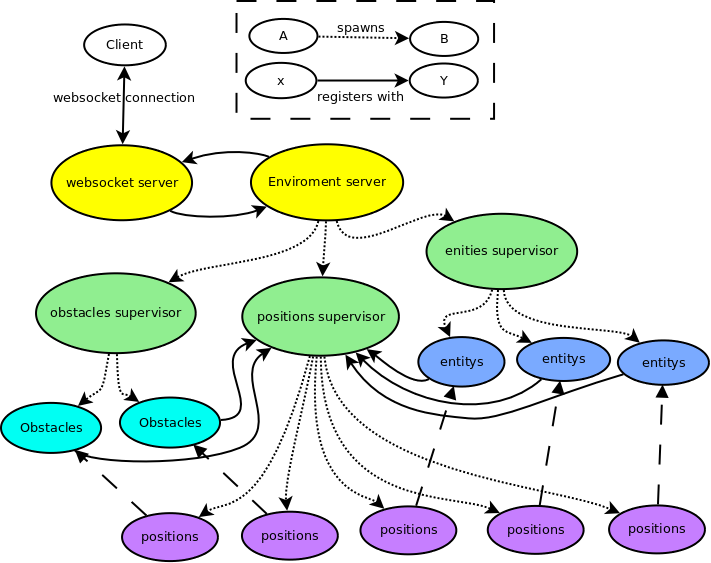
\includegraphics[width=0.8\textwidth]{img/HighLevelProcess.png}
\caption{Initial, obsolete, system design}
    \label{fig:Initial system design}
\end{figure}
As this early system diagram shows, we had planned for positions (represented as some kind of co-ordinate data) to be separate processes which would be generic and used by different "classes" of entities. Thankfully we revised this design further before we began to implement such a system.
The group would like to thank Dr F Barnes, for his input in our system revision. Dr Barnes, remarked that our design was similar to an early iteration of a concurrent flocking program he had worked on and provided us with a description of the system used by his program which greatly influenced our subsequent revisions.

\subsection{The Tile-Viewer model}
\label{tile_viewer_diagram}
Our revised design employed a system of concurrent tiles used to model space, we abandoned the idea of positions-as-processes, each tile would keep a list of the positions of entities on it and each entity would keep a record of it's own position and the address of the tile it currently occupies. Additional viewer process would be created to contain lists of cross-tile data, allowing entities to "see" into neighbouring tiles. An entity requests it's sensory data from its tile's corresponding viewer and a tile updates all its neighbouring viewers with the positions of entities it contains. This duplication of data allows us to maintain a high level of concurrency in the simulation, reducing potential message-passing bottle necks. Each tile has its own corresponding viewer, but this viewer additionally contains the data of neighbouring tiles which report to it.
\begin{figure}[h]
  \centering
  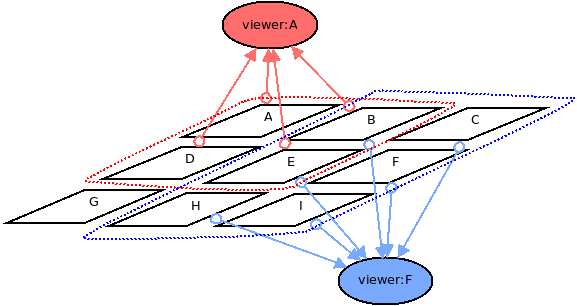
\includegraphics[width=0.8\textwidth]{img/tile_to_viewer_map.png}
\caption{Tile-Viewer System}
    \label{fig:Tile-Viewer System}
\end{figure}
The viewer corresponding to Tile:A (which would be Viewer:A) contains all the data from tiles A,B,D and E. When an entity on Tile:A needs information about its surroundings it calls on Viewer:A. This system allows an entity in the bottom-left corner of Tile:A to be aware of the contents of Tile:E. Viewer:F duplicates the data from Tiles B and E but entities calling on Viewer:F never receive data about the contents of Tile:A.

When an entity decides to move a negotiation takes place between the Tile and the entity; details of this negotiation can be found in section \ref{viewer_intro} but are summarised below.
\begin{enumerate}
\item{Entity informs its Tile of its preferred move}
\item{Tile informs entity of new position and which tile corresponds to that position.}
\end{enumerate}
crucially the tile computes the final position of the entity, this system allows the tile to handle collision. The potential for two entities to move simultaneously into the same space is avoided. This is in-keeping with our design goal of realism.

Our final system architecture (fig:\ref{fig:Zombie, Tile-Viewer Relationship}) also follows the general Open Telecom Platform (OTP) pattern using a supervisor-process hierarchy, further details of this OTP design pattern can be found in Section \ref{otp_description}
\begin{figure}[h]
  \centering
  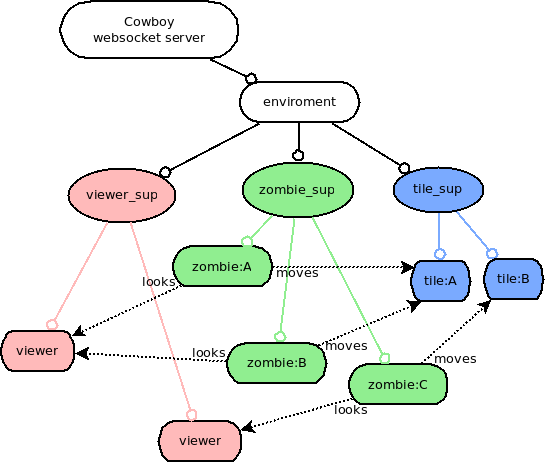
\includegraphics[width=0.8\textwidth]{img/system.png}
\caption{Zombie, Tile-Viewer Relationship}
    \label{fig:Zombie, Tile-Viewer Relationship}
\end{figure}

\clearpage
\endinput
